\apendice{Planificación del proyecto}

Este proyecto de investigación se desarrolla sobre la base del trabajo llevado a cabo durante la asignatura I+D+i en Informática del Máster en Ingeniería Informática de la Universidad de Valladolid, donde se realizó una revisión del Estado del Arte relativo a la estimación de profundidad monocular. Por lo tanto, la planificación planteada no incluye esta primera etapa.

Las tareas planificadas (T) para este Trabajo Fin de Máster, se han agrupado en paquetes de trabajo (PT) en base a su similitud. En la \Cref{fig:cronograma} se puede encontrar tanto la lista de tareas planteadas, como la asignación de recursos temporales a cada una de ellas.

\begin{figure}[H]
\centering
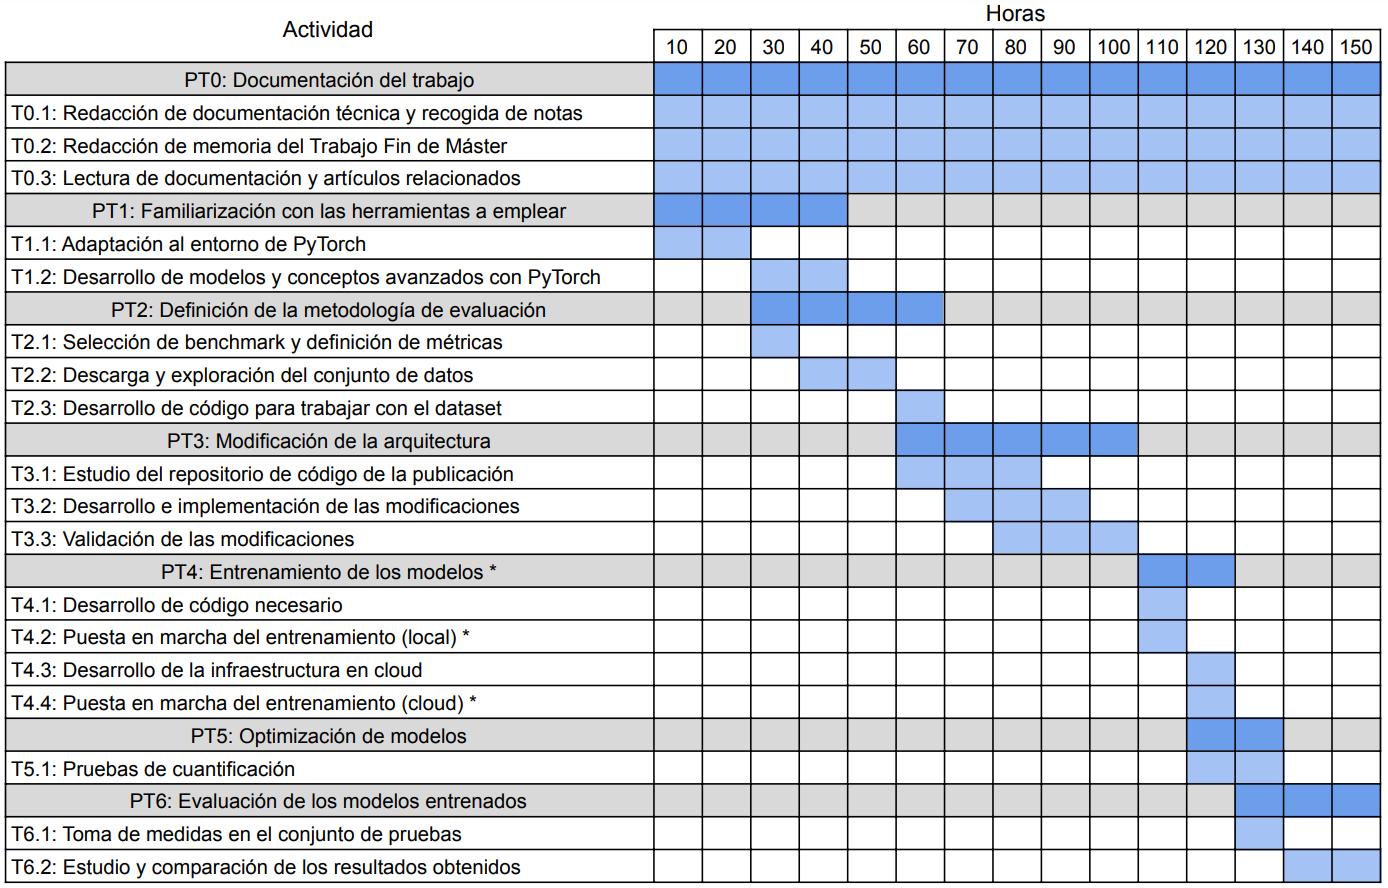
\includegraphics[width=\textwidth]{imagenes/planificacion.png}
\caption{Cronograma del proyecto.}
\label{fig:cronograma}
\end{figure}

(*) Cabe mencionar que el entrenamiento de los modelos ha sido un proceso especialmente largo, y por lo tanto se ha intentado en la medida de lo posible aprovechar este tiempo para la redacción de la documentación y las pruebas de cuantificación de modelos. 